\chapter{Resultados}

\section{Resultados de Simulação Computacional}

\subsection{Inversor isolado da rede elétrica}

\subsection{Inversor como STATCOM}

\subsection{Inversor conectado ao conversor \textit{boost}}

Nesta etapa de simulação, o objetivo foi verificar se o inversor trifásico, juntamente com sua malha de controle, conseguiam realizar transmissão de potência ativa do barramento CC para a rede elétrica. 
Para isto, conectou-se o do barramento de CC à um conversor do tipo \textit{boost}, que injetava corrente no barramento.
O inversor, de forma a manter a tensão no barramento CC constante, realizava as iterações em seu algorítmo de controle de forma a injetar na rede elétrica a corrente recebida.
A Fig. \ref{fig:sim-circuito-inversor-boost} mostra o circuito utilizado.

\begin{figure}[!hbt]
	\begin{center}
    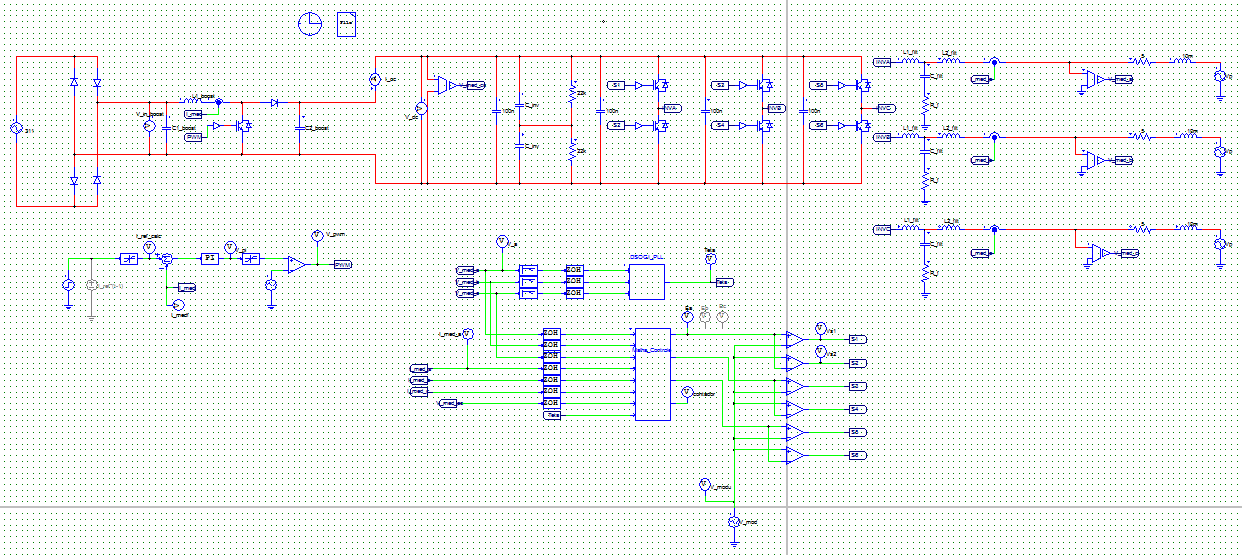
\includegraphics[width=\textwidth]{figuras/sim_figures/sistema_completo/montagem/sistema_completo.PNG}    \centering
    \caption{Circuito do inversor conectado com o conversor \textit{boost}, juntamente com os blocos de controle no software PSIM}
    \label{fig:sim-circuito-inversor-boost}
    \end{center}
\end{figure}

A tensão de referência definida para o barramento CC foi de 700 V. Desta forma, esperou-se que, apesar das pertubações a serem inseridas no sistema, este conseguisse estabilizar a tensão do barramento CC pŕoximo a tensão de referência após alguns segundos. 
Inicialmente o sistema foi inicializado sem nenhuma injeção de potência no barramento CC e permaneceu assim até os 4 segundos. Após, isso iniciou-se a injeção de potência através do conversor \textit{boost}, que foi programado para injetar 10 A de corrente.

Pode-se verificar na Fig. \ref{fig:sim-tensao-barramento} a estabilização de tensão no barramento CC. 
Antes dos 4 segundos, o sistema passou por um transitório mas conseguiu manter a tensão no barramento próximo de 700 V. 
Após isto, houve a inserção de corrente pelo \textit{boost}, que provocou uma pertubação, de forma a elevar a tensão sobre o \textit{link} capacitivo do barramento.
De forma a estabilizar esta tensão, o sistema começou a fornecer potência à rede elétrica de modo a manter a tensão CC próximo a seu valor de referência.

\begin{figure}[!hbt]
	\begin{center}
    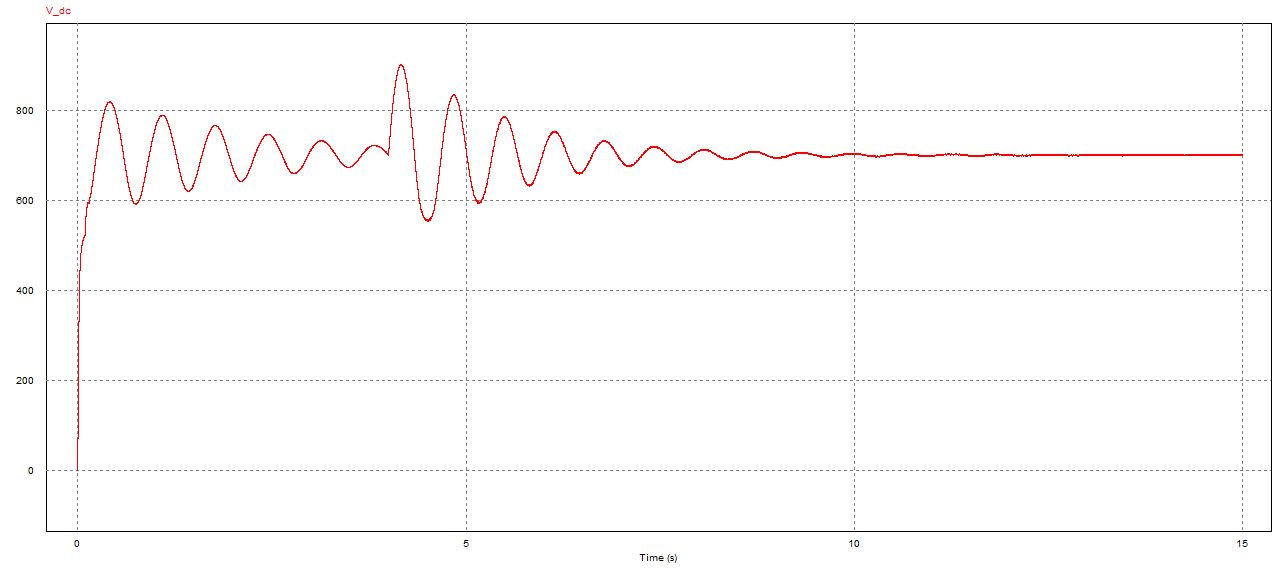
\includegraphics[width=\textwidth]{figuras/sim_figures/sistema_completo/tensao_barramento.PNG}
    \caption{Tensão no barramento CC. A tensão de referência foi definida como 700 V. Inicialmente o sistema foi inicializado sem nenhuma injeção de potência no barramento, como pode-se verificar antes dos 4 segundos. Depois, acontece uma pertubação devido a inserção de potência, mas este estabiliza-se próximo a tensão de referência após alguns segundos}
    \label{fig:sim-tensao-barramento}
    \end{center}
\end{figure}

A Fig. \ref{fig:sim-tensao-saida-inversor} mostra as tensões sintetizadas na saída do inversor, após o filtro $L_2$.
Ao se verificar o expectro em frequência da tensão sintetizada na fase $V_A$, é possível ver que existem harmônicas perto da frequência de chaveamento, mas que não produzem alterações significativas na tensão de saída. 
Verifica-se ainda que houve a sintetização correta das tensões em cada fase.

Já a Fig. \ref{fig:sim-corrente-saida-inversor} mostra as correntes geradas após a inserção de potência pelo \textit{boost} no barramento CC.
O expectro em frequência da corrente produzida na fase A denominada $I_A$ mostra que existem harmônicas de baixa frequência, de quinta e sétima ordem, mas que não provocam alterações significativas na corrente produzida.
Ainda é possível verificar o envio correto das três correntes para a rede elétrica.

\begin{figure}[!hbt]
	\centering
	\begin{subfigure}[b]{0.5\textwidth}
		\centering
		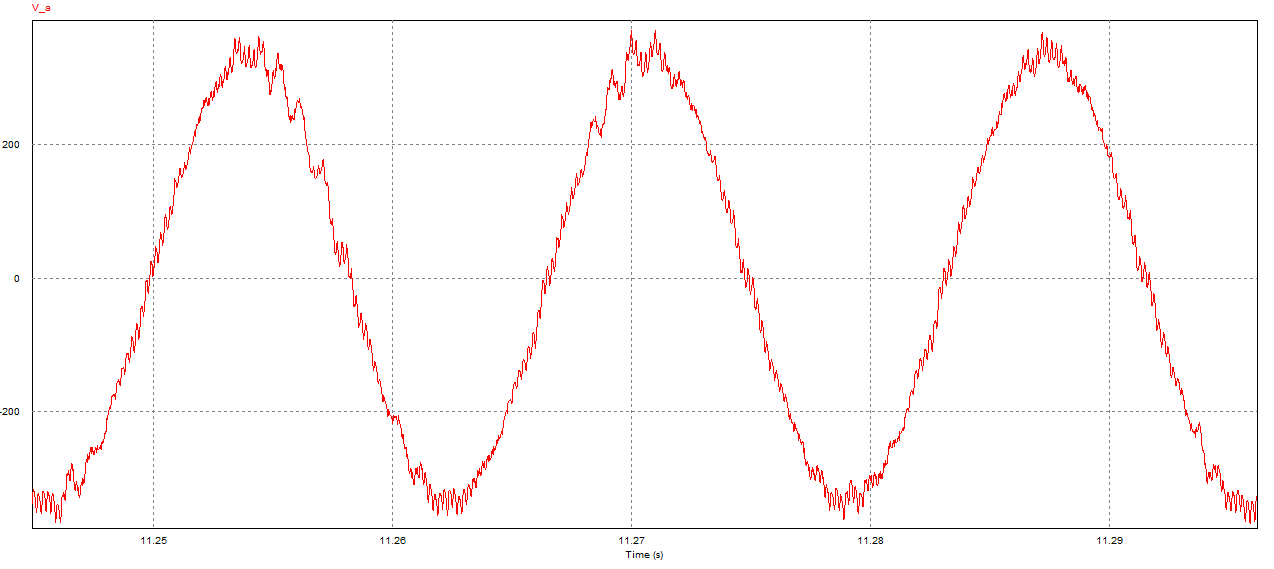
\includegraphics[width=\textwidth]{figuras/sim_figures/sistema_completo/tensao_saida_inversor_2.PNG}
		\caption{Tensão de saída sintetizada para a fase A}
   \end{subfigure}

   \begin{subfigure}[b]{0.5\textwidth}
		\centering
		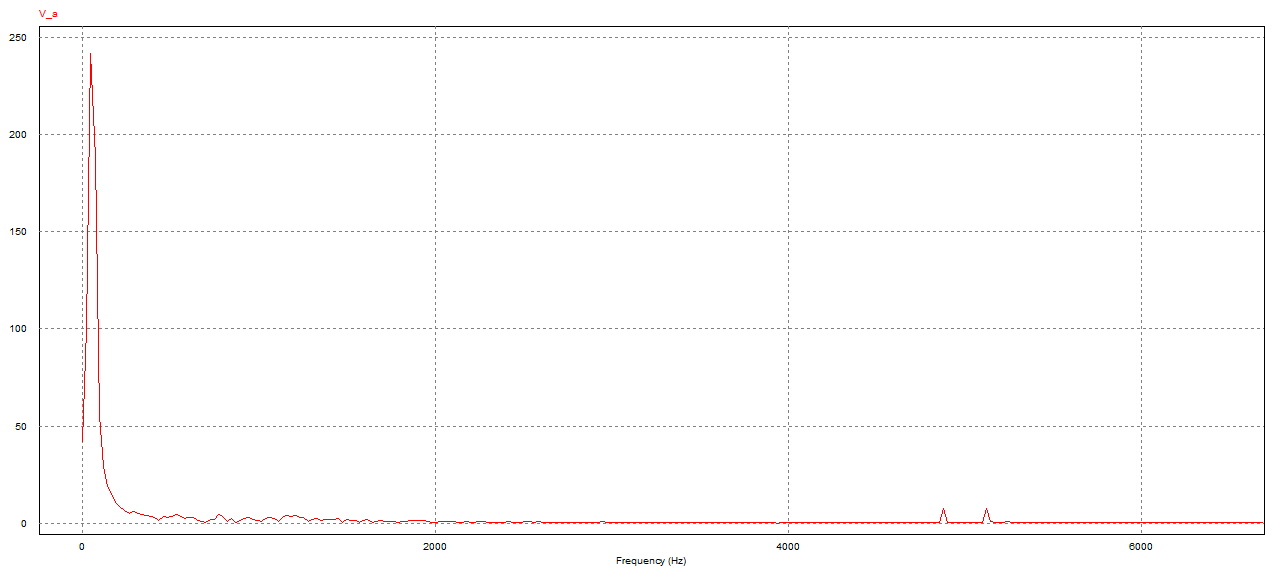
\includegraphics[width=\textwidth]{figuras/sim_figures/sistema_completo/tensao_saida_inversor_fft.PNG}
		\caption{Expectro em frequência da tensão sintetizada na fase A. Os harmônicos de alta frequência próximos a frequência de chaveamento de 5 kHz sofreram uma boa atenuação}
   \end{subfigure}

	\begin{subfigure}[b]{0.5\textwidth}
		\centering
		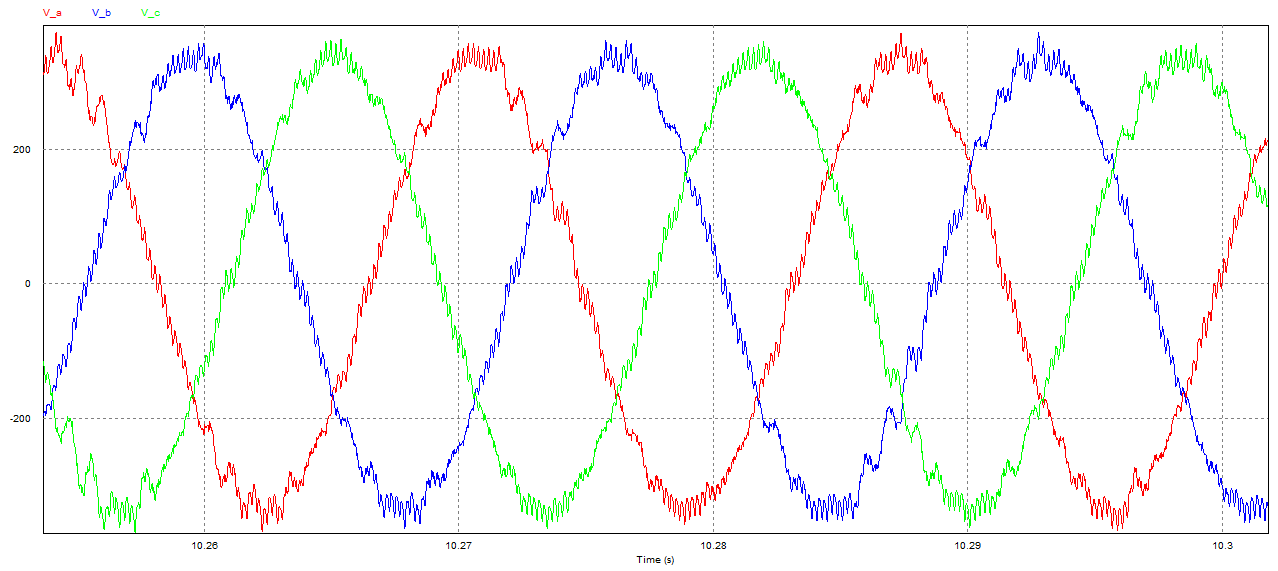
\includegraphics[width=\textwidth]{figuras/sim_figures/sistema_completo/tensao_saida_inversor_4.PNG}
		\caption{Tensões de saída sintetizadas para as fases A, B e C}
	\end{subfigure}
    \caption{Análise das tensões de saída sintetizadas após o filtro LCL}
    \label{fig:sim-tensao-saida-inversor}
\end{figure}

\begin{figure}[!hbt]
	\centering
	\begin{subfigure}[b]{0.5\textwidth}
		\centering
		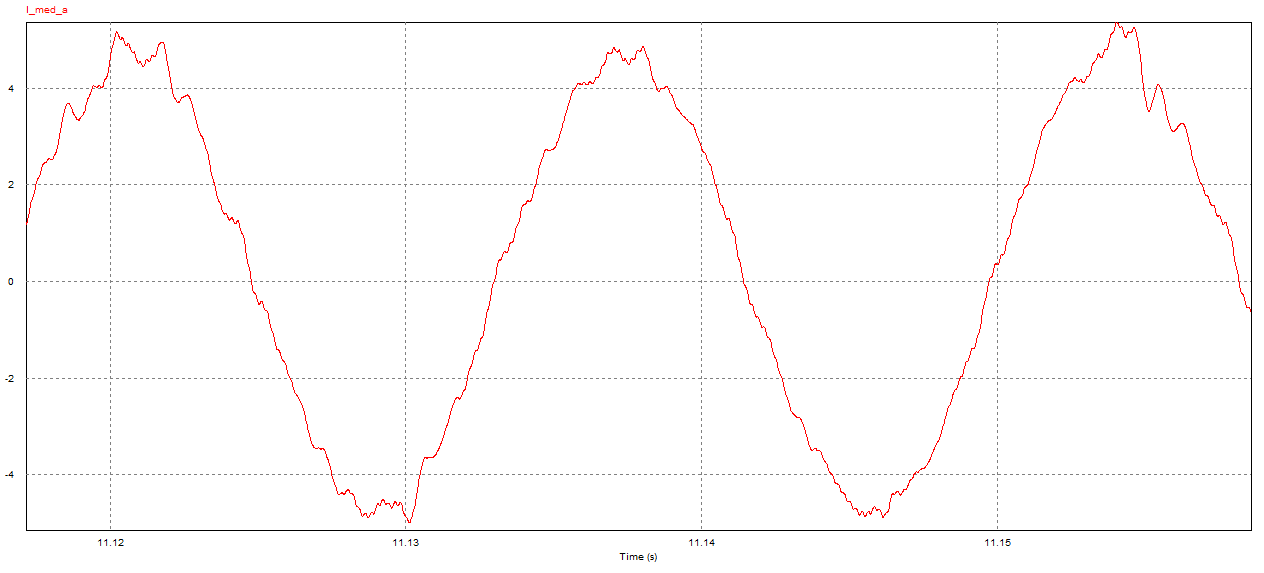
\includegraphics[width=\textwidth]{figuras/sim_figures/sistema_completo/corrente_saida_inversor_1.PNG}
		\caption{Corrente de saída na fase A}
    \end{subfigure}

    \begin{subfigure}[b]{0.5\textwidth}
		\centering
		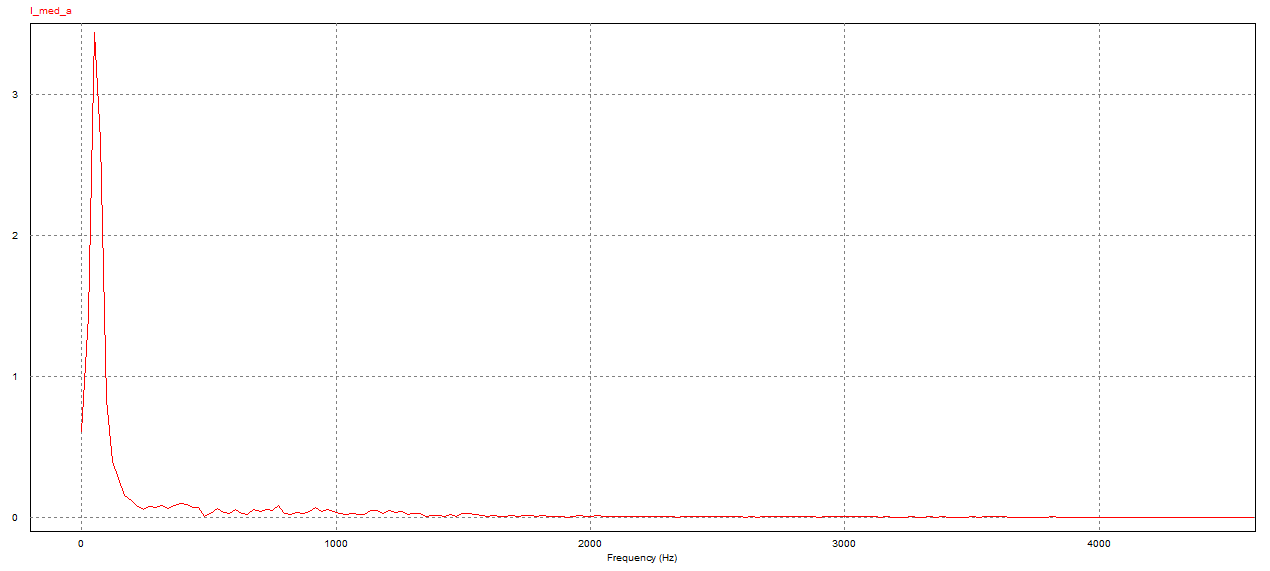
\includegraphics[width=\textwidth]{figuras/sim_figures/sistema_completo/corrente_saida_inversor_fft.PNG}
		\caption{Expectro em frequência da corrente na fase A. Os harmônicos de baixa frequência também sofreram uma boa atenuação}
    \end{subfigure}

	\begin{subfigure}[b]{0.5\textwidth}
		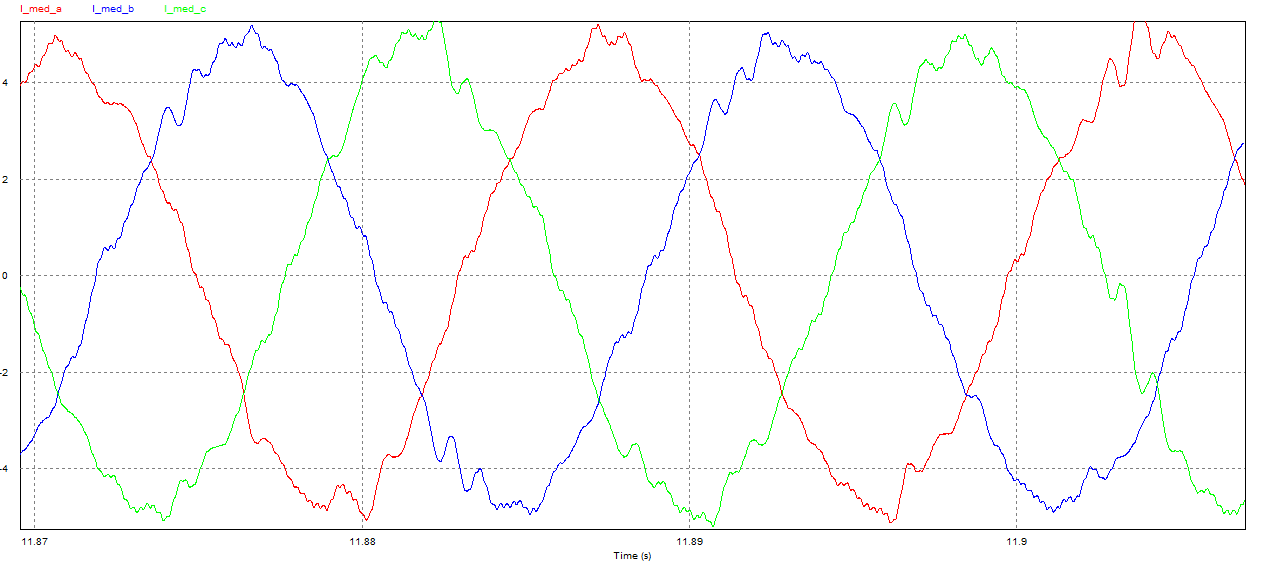
\includegraphics[width=\textwidth]{figuras/sim_figures/sistema_completo/corrente_saida_inversor_2.PNG}
		\caption{Correntes de saída para as fases A, B e C}
	\end{subfigure}
    \caption{Análise das corrente de saída após o filtro LCL. Estes resultados foram obtidos após a inserção de corrente pelo conversor \textit{boost} no barramento CC}
    \label{fig:sim-corrente-saida-inversor}
\end{figure}

Na Fig. \ref{fig:sim-tensao-corrente-boost} pode-se verificar os valores de tensão e de corrente na entrada do conversor \textit{Boost}.
É possível ver que a tensão na entrada do conversor é aproximadamente 250 V, e a corrente de entrada aproximadamente 10 A, produzindo desta forma uma potência de entrada $P_{entrada}$ = 2500 W.

Utilizando as Figs. \ref{fig:sim-tensao-saida-inversor} e \ref{fig:sim-corrente-saida-inversor} verifica-se que a tensão de pico é aproximadamente 311 V e que a corrente de pico é aproximadamente 5,2 A.
Desta forma, convertendo para RMS, temos que a tensão RMS é 219,91 V e a corrente RMS 3,7 A. A potência de saída trifásica é, portanto, $P_{saída}$ = $ 3 \times 219,9 \times 3,7$ = 2441 W, mostrando, portanto, que a potência foi transferida, com algumas perdas, para a rede elétrica.

\begin{figure}[!hbt]
	\centering
	\begin{subfigure}[b]{0.5\textwidth}
		\centering
		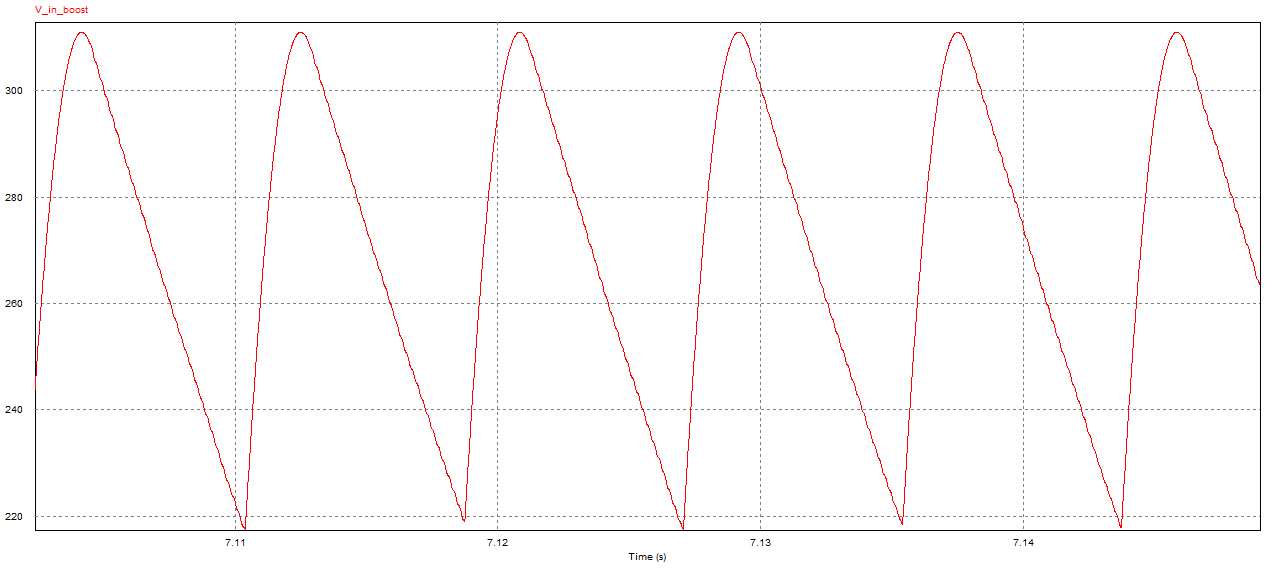
\includegraphics[width=\textwidth]{figuras/sim_figures/sistema_completo/tensao_entrada_boost_2.PNG}
		\caption{Tensão na entrada do conversor \textit{Boost}. A tensão média na entrada foi de 250 $V_{DC}$}
	\end{subfigure}
	
	\begin{subfigure}[b]{0.5\textwidth}
		\centering
		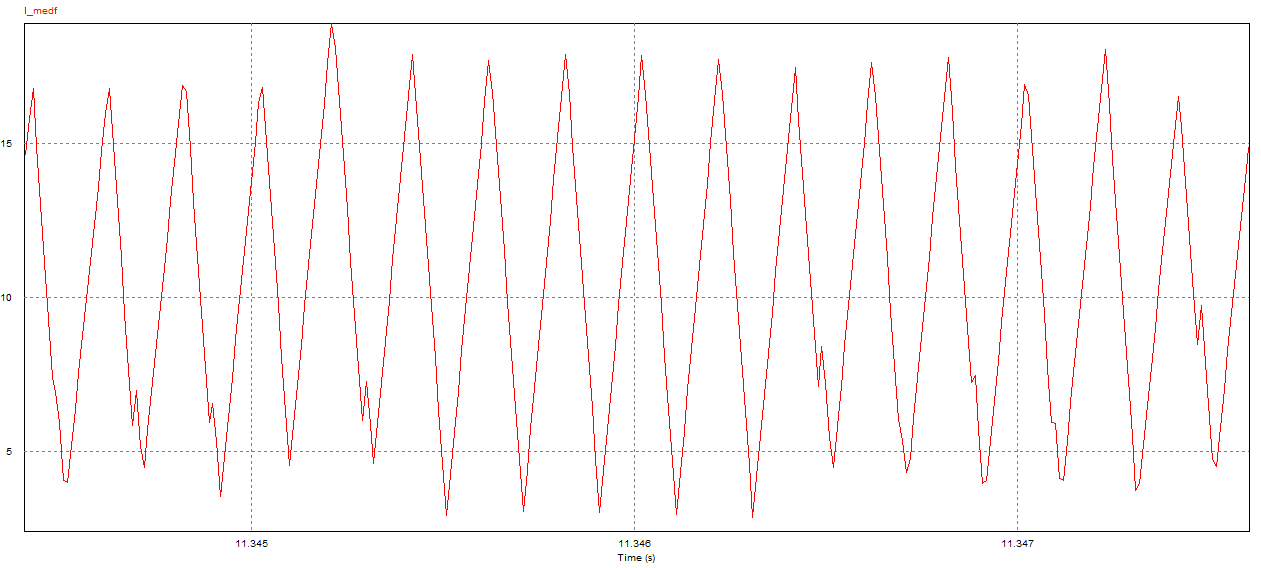
\includegraphics[width=\textwidth]{figuras/sim_figures/sistema_completo/corrente_entrada_boost_2.PNG}
		\caption{Corrente medida na entrada do conversor \textit{Boost}. A corrente média foi de 10 A}
	\end{subfigure}

	\caption{Verificação da tensão e corrente de entrada no conversor \textit{Boost} para cálculo da potência de entrada do sistema}
    \label{fig:sim-tensao-corrente-boost}
\end{figure}

\subsection{Comportamento do inversor com a inserção de potência variável no barramento CC}

\section{Resultados Experimentais}

A Fig. \ref{fig:res-bancada-inversor} apresenta a montagem experimental realizada para validação da bancada.
Esta montagem foi realizada utilizando o inversor desacoplado da rede elétrica, de forma que fosse possível validar
os algoritmos de sincronização e de controle. Os testes com o inversor trifásico acoplado à rede elétrica como STATCOM e
utilizando o conversor \textit{boost} ainda estão sendo realizados e não serão abordados neste trabalho.

\begin{figure}[!hbt]
	\begin{center}
    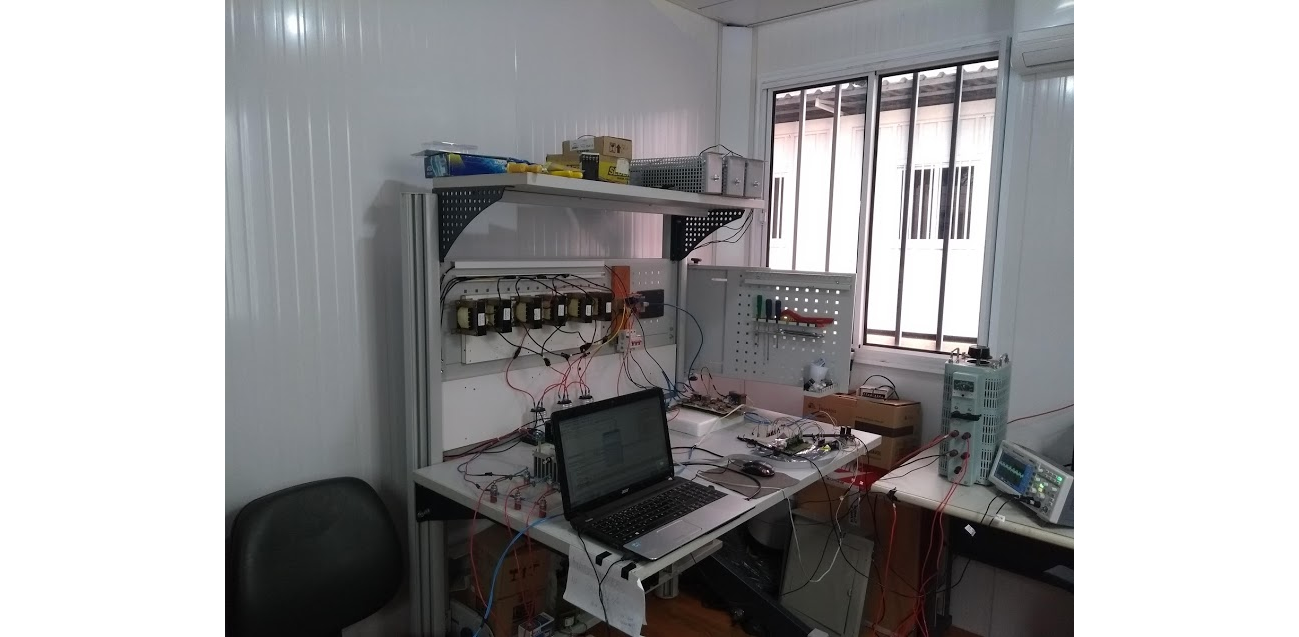
\includegraphics[width=\textwidth]{figuras/resultados-montagem-laboratorial.png}
    \caption{Bancada do inversor trifásico com seus componentes}
    \label{fig:res-bancada-inversor}
    \end{center}
\end{figure}

\subsection{Obtenção e calibração dos sinais de tensão da rede}

A Fig. \ref{fig:res-tensao-va-vb-bc} mostra as tensões da rede elétrica após a etapa de condicionamento de sinais.
Para que as tensões e correntes pudessem ser quantizadas corretamente pelo microcontrolador, 
uma etapa de ajustes finos da placa de condicionamento de sinais foi necessária para que os sinais estivessem dentro da faixa de amostragem do conversor A/D.
Mais especificamente, foi realizado um ajuste através de um \textit{trimpot} que regulava o nível DC dos sinais na entrada do DSP.
Além disso, foi necessário se atentar para a correta sequência de fase da rede elétrica.

\begin{figure}[!hbt]
	\centering
	\begin{subfigure}[b]{0.49\textwidth}
		\centering
		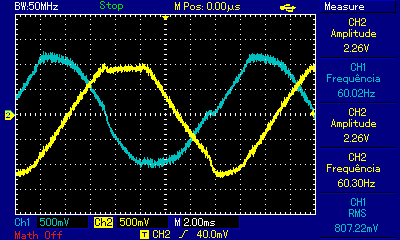
\includegraphics[width=\textwidth]{figuras/resultados_tensao_va_vb.png}
		\caption{Tensões $V_A$ (canal 1) e $V_B$ (canal 2) após o processamento pela placa de condionamento de sinais e trandutores}
	\end{subfigure}
	\begin{subfigure}[b]{0.49\textwidth}
		\centering
		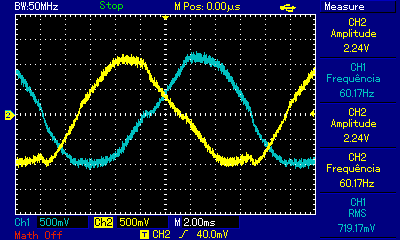
\includegraphics[width=\textwidth]{figuras/resultados_tensao_va_vc.png}
		\caption{Tensões $V_A$ (canal 1) e $V_C$ (canal 2) após o processamento pela placa de condionamento de sinais e trandutores}
	\end{subfigure}

	\caption{Verificação dos sinais respectivos às tensões da rede elétrica após a placa de condicionamento de sinais}
    \label{fig:res-tensao-va-vb-bc}
\end{figure}

\subsection{Sincronização com a rede elétrica}

A Fig. \ref{fig:res-sincronizacao} mostra a correta sincronização do algoritmo do DSOGI-PLL. 
A GPIO10 do DSP foi configurado como saída digital e no semiciclo positivo da senoide da rede elétrica era acionado (3,3 V) e no semiciclo negativo desativado (0 V).
O ângulo de fase da rede elétrica foi utilizado para o correto acionamento do GPIO, atestando assim o funcionamento do algoritmo em C do DSOGI-PLL no DSP.

\begin{figure}[!hbt]
	\begin{center}
    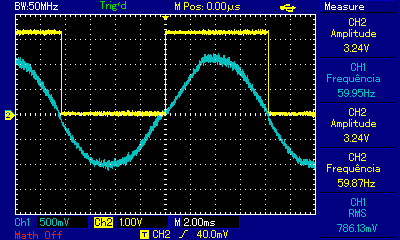
\includegraphics[width=0.4\textwidth]{figuras/resultados_sincronizacao.png}
	\caption{Resultado de sincronização do sistema com a rede elétrica. O canal A do osciloscópio estava conectado ao sensor de tensão da fase $V_A$ da rede elétrica e o canal B estava conectado ao GPIO 10 do DSP.}
    \label{fig:res-sincronizacao}
    \end{center}
\end{figure}

\subsection{Verificação do SPWM}

Para realização do chaveamento dos IGBTs do inversor, o DSP TMS320F28335 dispõe
de um módulos conhecido como \textit{enhanced Pulse Width Modulation} - ePWM, a qual dispõem de diversas configurações aplicadas à sistemas de potência.
Desta forma, a frequência de chaveamento foi configurada para 5 kHz e o tempo morto entre os acionamentos dos IGBTs para 10 $\mu s$. 
A Fig. \ref{fig:res-pwm} mostra os resultados obtidos. Pode-se verificar que as especificações requeridas foram atendidas.

\begin{figure}[!hbt]
	\centering
	\begin{subfigure}[b]{0.49\textwidth}
		\centering
		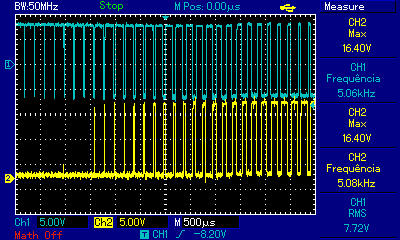
\includegraphics[width=\textwidth]{figuras/resultados_pwm1_1.png}
		\caption{Forma de onda do PWM trifásico}
	\end{subfigure}
	\begin{subfigure}[b]{0.49\textwidth}
		\centering
		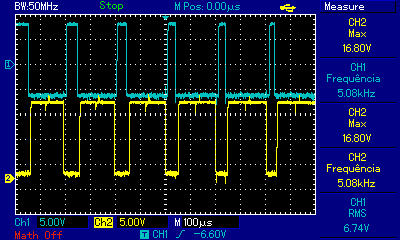
\includegraphics[width=\textwidth]{figuras/resultados_pwm2_1.png}
		\caption{Aproximação na forma de onda}
	\end{subfigure}
	\begin{subfigure}[b]{0.49\textwidth}
		\centering
		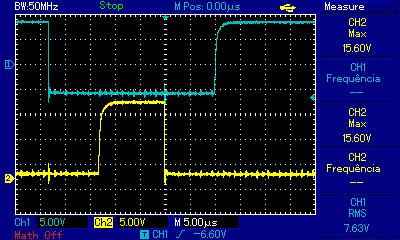
\includegraphics[width=\textwidth]{figuras/resultados_tempo_morto1.png}
		\caption{Aproximação mais detalhada para demonstrar o tempo morto configurado}
	\end{subfigure}
	\begin{subfigure}[b]{0.49\textwidth}
		\centering
		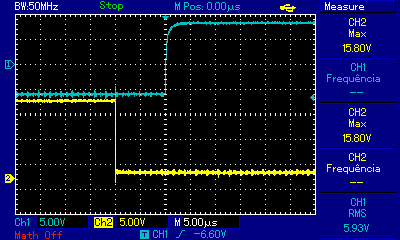
\includegraphics[width=\textwidth]{figuras/resultados_tempo_morto2.png}
		\caption{Verificação do tempo morto de 10 $\mu s$}
	\end{subfigure}
	\caption{Sinal de PWM amplificado após a placa de conversão dos sinais de 3,3V para 15V. O módulo ePWM do DSP foi configurado para ter uma frequência de chaveamento de 5 kHz e tempo morto de 10 $\mu s$ entre as bordas de subida e descida dos sinais de acionamento de cada IGBT}
    \label{fig:res-pwm}
\end{figure}

\subsection{Validação da malha de controle de corrente}

Para validação da malha de controle de corrente, foi criado um teste em C em que a corrente de referência em eixo direto $I_{d,ref}$ 
foi variada a cada 5 segundos, de forma que esta era inicializada em 0,3 A, após 5 segundos, passava para 0,6 A e assim sucessivamente,
até atingir 1,5 A, e depois voltava para 0,3 A, em um esquema de escada.

Assim, verificou-se a corrente enviada para os resistores de 100 $\Omega$ com o alicate amperímetro e a Tab. \ref{tab:res-controle-corrente} foi montada.
Pode-se verificar que a corrente medida no alicate amperímetro tem uma amplitude próxima da corrente desejada, demonstrando assim que a malha de controle de corrente
estava funcionando. Os erros entre os valores medidos e esperados são devidos, principalmente, as perdas nos componentes elétricos.

A Fig. \ref{fig:res-controle-corrente} mostra a variação na amplitude da corrente medida pelo trandutor e placa de condionamento de sinais a cada 5 segundos, 
e a Fig. \ref{fig:res-escada-corrente} mostra a variação da amplitude de corrente no tempo demonstrando assim o correto controle da malha.

\begin{table}[h]
	\centering
	\caption{Resultados para atestar o funcionamento da malha de controle de corrente. Os passos foram dados a cada 5 segundos.}
	\label{tab:res-controle-corrente}
	
	\begin{tabular}{m{5cm}m{5cm}m{5cm}}
		\toprule
		\multicolumn{3}{c}{\textbf{Tensão no barramento CC:} 308 V} \\
		\textbf{Corrente Esperada (A)} & \textbf{Corrente Medida (A)} & \textbf{Tensão sintetizada pelo inversor (V)}\\
		\midrule
		\multicolumn{1}{c}{0,3} & \multicolumn{1}{c}{0,225} & \multicolumn{1}{c}{40} \\
		\multicolumn{1}{c}{0,6} & \multicolumn{1}{c}{0,460} & \multicolumn{1}{c}{82} \\
		\multicolumn{1}{c}{0,9} & \multicolumn{1}{c}{0,693} & \multicolumn{1}{c}{124} \\
		\multicolumn{1}{c}{1,2} & \multicolumn{1}{c}{0,930} & \multicolumn{1}{c}{167} \\
		\multicolumn{1}{c}{1,5} & \multicolumn{1}{c}{1,173} & \multicolumn{1}{c}{209} \\
		\bottomrule
	\end{tabular}
\end{table}

\begin{figure}[!hbt]
	\centering
	\begin{subfigure}[b]{0.49\textwidth}
		\centering
		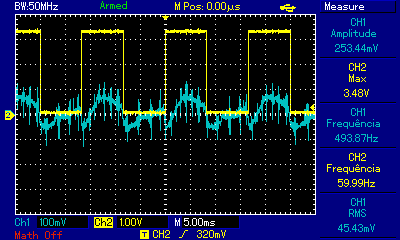
\includegraphics[width=\textwidth]{figuras/resultados_controle_corrente_0_3.png}
		\caption{Resultado para $I_{d,ref}$ = 0,3 A}
	\end{subfigure}
	\begin{subfigure}[b]{0.49\textwidth}
		\centering
		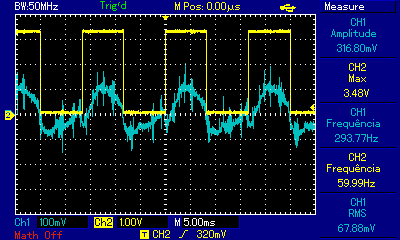
\includegraphics[width=\textwidth]{figuras/resultados_controle_corrente_0_6.png}
		\caption{Resultado para $I_{d,ref}$ = 0,6 A}
	\end{subfigure}
	\begin{subfigure}[b]{0.49\textwidth}
		\centering
		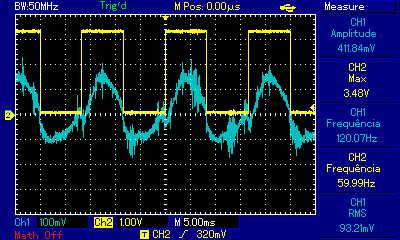
\includegraphics[width=\textwidth]{figuras/resultados_controle_corrente_0_9.png}
		\caption{Resultado para $I_{d,ref}$ = 0,9 A}
	\end{subfigure}
	\begin{subfigure}[b]{0.49\textwidth}
		\centering
		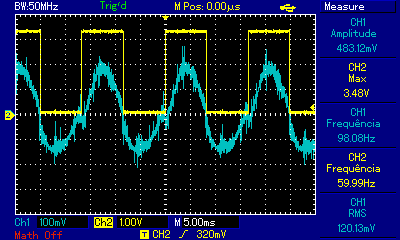
\includegraphics[width=\textwidth]{figuras/resultados_controle_corrente_1_2.png}
		\caption{Resultado para $I_{d,ref}$ = 1,2 A}
	\end{subfigure}
	\begin{subfigure}[b]{0.49\textwidth}
		\centering
		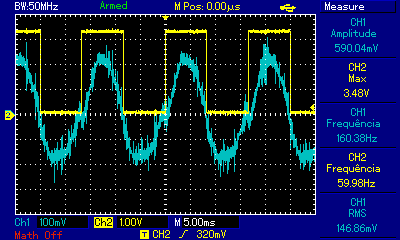
\includegraphics[width=\textwidth]{figuras/resultados_controle_corrente_1_5.png}
		\caption{Resultado para $I_{d,ref}$ = 1,5 A}
	\end{subfigure}
	\caption{Verificação do aumento da amplitude no sinal de corrente, mostrando que o controle de corrente está sendo realizado pelo sistema. No canal 1 está o sinal de corrente lido após a placa de condicionamento de sinais e no canal 2 o GPIO10, que é ativado nos semiciclos positivos da PLL, mostrando que a corrente está em fase com a tensão da rede.}
    \label{fig:res-controle-corrente}
\end{figure}

\begin{figure}[!hbt]
	\begin{center}
    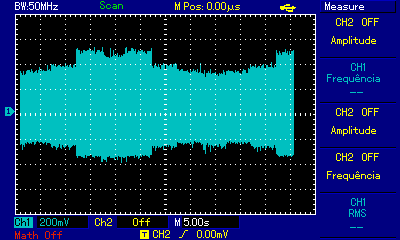
\includegraphics[width=0.4\textwidth]{figuras/resultados_escada_corrente.png}
	\caption{Escada de corrente no tempo mostrando a variação de amplitude a cada 5 segundos}
    \label{fig:res-escada-corrente}
    \end{center}
\end{figure}
